\documentclass[12pt, a4paper]{article}

\usepackage[utf8]{inputenc}
\usepackage[english, russian]{babel}
\usepackage{fancyhdr}
\usepackage{amsmath}
\usepackage{amsthm}
\usepackage{float}
\usepackage{graphicx}
\graphicspath{ {./} }
\usepackage{tabularx}
\newcolumntype{L}{>{\raggedright\arraybackslash}X}
\usepackage{pgfplots}
\usepackage{float}
\usepackage{xcolor}
\usepackage{hyperref}
\usepackage{multirow}
\usepackage{diagbox}
\pgfplotsset{width=\textwidth*0.8, compat=1.13}

\usepgfplotslibrary{external}
\usepgfplotslibrary{fillbetween}
\usepgfplotslibrary{statistics}
\usetikzlibrary{patterns.meta}


\graphicspath{{./}}
\newcommand{\Mod}[1]{\ \mathrm{mod}\ #1}

\usepackage[a4paper, margin=1.5cm]{geometry}

\usepackage{titlesec}
\titlelabel{\thetitle.\quad}

\pagestyle{plain}

\fancypagestyle{firstpage}{%
  \chead{
  МИНИСТЕРСТВО НАУКИ И ВЫСШЕГО ОБРАЗОВАНИЯ РОССИЙСКОЙ ФЕДЕРАЦИИ 
ФЕДЕРАЛЬНОЕ ГОСУДАРСТВЕННОЕ АВТОНОМНОЕ  
ОБРАЗОВАТЕЛЬНОЕ УЧРЕЖДЕНИЕ ВЫСШЕГО ОБРАЗОВАНИЯ\bigskip

«Национальный исследовательский университет ИТМО»\bigskip

ФИЗИЧЕСКИЙ ФАКУЛЬТЕТ 
}
\fancyfoot[CO]{Санкт-Петербург, 2023}%
}



\definecolor{aqua}{HTML}{003844}
\definecolor{peri}{HTML}{5EB1BF}
\definecolor{royal_blue}{HTML}{0A2463}
\definecolor{periwinkle}{HTML}{D8DCFF}
\definecolor{cerulean}{HTML}{247BA0}
\definecolor{bloodred}{HTML}{690500}
\definecolor{imperial_red}{HTML}{FB3640}
\definecolor{purple}{HTML}{511730}
\definecolor{tangerine}{HTML}{FFA781}

\definecolor{blue1}{HTML}{142459}
\definecolor{blue2}{HTML}{176BA0}
\definecolor{blue3}{HTML}{19AADE}
\definecolor{blue4}{HTML}{1AC936}
\definecolor{blue5}{HTML}{1DE4BD}
\definecolor{blue6}{HTML}{6DF0D2}

\definecolor{pink1}{HTML}{29066B}
\definecolor{pink2}{HTML}{7D3AC1}
\definecolor{pink3}{HTML}{AF4BCE}
\definecolor{pink4}{HTML}{DB4CB2}
\definecolor{pink5}{HTML}{EB548C}
\definecolor{pink6}{HTML}{EA7369}
\newtheorem*{task}{Условие}
\newtheorem*{finish}{Заключение}

\counterwithin{figure}{section}

%\tikzexternalize
\begin{document}
\newgeometry{top=1.6cm,bottom=1.6cm, left = 1.2cm, right = 1.2cm}

\topskip0pt
\vspace*{0.25\textheight}
\begin{center}
\textbf{\LARGE РАБОЧИЙ ПРОТОКОЛ И ОТЧЁТ }

\LARGE по лабораторной работе №1.13

\LARGE <<Изучение прецессии гироскопа>>

\end{center}
\vspace*{5cm}
\begin{flushright}
\begin{minipage}{.33\linewidth}
\textit{\textbf{Выполнил:}}\\
Хороших Дмитрий - P3217\\
\textit{\textbf{Преподаватель:}}\\
Хуснутдинова Наира\\ Рустемовна
\end{minipage}
\end{flushright}


\thispagestyle{firstpage}
\newpage
\tableofcontents

\restoregeometry
\section{Введение}
\begin{enumerate}
\item Цель работы:

Пронаблюдать прецессии гироскопа. Экспериментально подтвердить линейную зависимость периода прецессии гироскопа от частоты вращения гироскопа вокруг оси симметрии. Экспериментально определить момент инерции гироскопа.
\item Задачи:
	\begin{enumerate}
		\item[1.]  Измерить период прецессии гироскопа.
		\item[2.] Измерить частоту вращения гироскопа вокруг своей оси.
		\item[3.] Рассчитать момент инерции гироскопа относительно оси вра-
щения, используя данные полученные в ходе экперимента. Сравнить полученный результат с моментом инерции гироскопа, рассчитанным теоретически.
	\end{enumerate}
		
\item Объект исследования:

Установка с гироскопом.

\item Схема установки:
\begin{figure}[H]
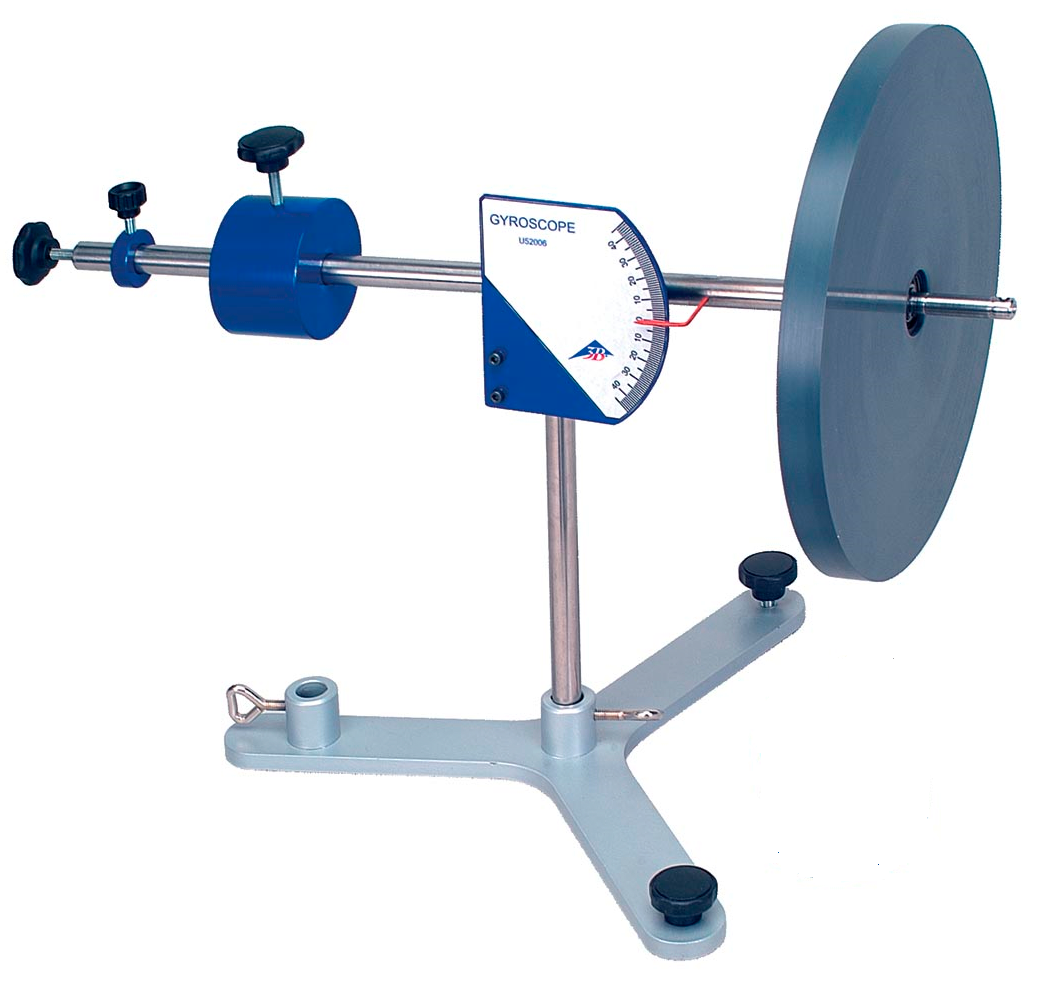
\includegraphics[width=0.5\textwidth]{gyro.png}
\centering
\caption{Гироскоп}
\end{figure}

Параметры гироскопа: масса маховика ($m$): 1.5 кг; радиус маховика ($R$): 12.5 см; расстояние от точки опоры оси вращения до места крепления дополнительных грузов ($l$): 22.5 см. 

\item Метод экспериментального исследования:

Многократный прямой замер периодов прецессии и частоты вращения маховика.

\item Рабочие формулы:

Связь периода прецессии с частотой вращения маховика:
\begin{equation}
T_{\text{пр}} = \frac{2\pi I}{mgl}\omega_{\text{ср}}
\end{equation}

Теоретический момент инерции гироскопа:
\begin{equation}
I_{\text{теор}} = \frac{mR^2}{2}
\end{equation}

\item Измерительные приборы:

\begin{table}[H]
\centering
\begin{tabular}{|l|l|l|l|l|}
\hline
№ п/п & Наименование & Тип & Используемый диапазон & Погрешность приб.\\
\hline
1 & Тахометр & Электронный & 0 - 9999 RPM  & 1 RPM\\
\hline
2 & Секундомер & Электронный & 0 - 9999 с & 0.01 с\\
\hline
3 & Весы & Электронный & 0 - 999 г. & 0.01 г.\\
\hline
\end{tabular}
\end{table}

\end{enumerate}
\section{Результаты измерений и их обработка}

Несколько раз измерим периоды прецессии и частоты вращения маховика для каждого набора грузов (от 1-го до 3-х). Рассчитаем среднюю частоту в ходе прецессии для каждого замера.


\begin{table}[H]
\begin{center}
\begin{tabular}{|c|c|c|c|c|}
\hline 
$m$, г & $\omega_1$, об./мин & $\omega_2$, об./мин & $\omega_{\text{ср}}$, об./мин & $T_\text{пр}$, с\\ 
\hline 
\multirow{5}{*}{$m_0$ + 1 $\cdot$ $m_1$} & 525.70 & 472.00 & 498.85 & 29.23\\ 
\cline{2-5} 
 & 401.80 & 375.40 & 388.60 & 23.43\\ 
\cline{2-5} 
 & 552.50 & 506.10 & 529.30 & 31.68\\ 
\cline{2-5} 
 & 402.30 & 374.20 & 388.25 & 23.42\\ 
\cline{2-5} 
 & 354.60 & 327.80 & 341.20 & 21.60\\ 
\cline{2-5} 
\hline 
\multirow{5}{*}{$m_0$ + 2 $\cdot$ $m_1$} & 565.40 & 523.70 & 544.55 & 17.78\\ 
\cline{2-5} 
 & 599.10 & 562.90 & 581.00 & 18.45\\ 
\cline{2-5} 
 & 413.10 & 393.80 & 403.45 & 12.98\\ 
\cline{2-5} 
 & 360.30 & 349.00 & 354.65 & 11.80\\ 
\cline{2-5} 
 & 513.60 & 492.80 & 503.20 & 16.28\\ 
\cline{2-5} 
\hline 
\multirow{5}{*}{$m_0$ + 3 $\cdot$ $m_1$} & 499.10 & 477.30 & 488.20 & 9.38\\ 
\cline{2-5} 
 & 589.00 & 562.40 & 575.70 & 12.30\\ 
\cline{2-5} 
 & 450.30 & 430.60 & 440.45 & 9.51\\ 
\cline{2-5} 
 & 469.60 & 450.00 & 459.80 & 10.33\\ 
\cline{2-5} 
 & 561.60 & 531.80 & 546.70 & 11.58\\ 
\cline{2-5} 
\hline 

\end{tabular}
\caption{Результаты прямых измерений частот маховика и периода прецессии.}
\label{tab:1}
\end{center}
\end{table}

Построим графики экспериментальной зависимости периода прецессии гироскопа от частоты вращения его маховика для каждого набора грузов.

\begin{figure}[H]
\centering
\begin{tikzpicture}
\begin{axis}[
	axis lines = left,
	ylabel = \(T \text{, с}\),
	xlabel = {\(\omega_{\text{ср}} \text{, рад/с}\)},
	ymin=0,	
	ymax=35,
	xmin=0,
	xmax=65,
	grid=both,
    grid style={line width=.1pt, draw=gray!10},
    major grid style={line width=.2pt,draw=gray!50},
    minor tick num=5,
	axis x line = bottom,
	axis line style ={line width = .3pt},
	legend style={at={(0.05, 0.9)},anchor=west}
	]


\addplot[only marks, blue1, mark size =2pt, mark=square*, error bars/.cd, y dir=both, y explicit, x dir=both, x explicit, error mark options={ blue1,mark size=0.4pt, line width=4pt }, error bar style={fill=blue1,scale=2, line width=1pt}] table [y = PERIOD, x = FREQ,  col sep=comma] {../period_by_freq1.csv}; 
\addplot[blue1, domain=0:65] {0.5738321552598661*x};
\addplot[only marks, blue2, mark size =2pt, mark=square*, error bars/.cd, y dir=both, y explicit, x dir=both, x explicit, error mark options={ blue2,mark size=0.4pt, line width=4pt }, error bar style={fill=blue2,scale=2, line width=1pt}] table [y = PERIOD, x = FREQ,  col sep=comma] {../period_by_freq2.csv}; 
\addplot[blue2, domain=0:65] {0.30872811757216323*x};
\addplot[only marks, blue3, mark size =2pt, mark=square*, error bars/.cd, y dir=both, y explicit, x dir=both, x explicit, error mark options={ blue3,mark size=0.4pt, line width=4pt }, error bar style={fill=blue3,scale=2, line width=1pt}] table [y = PERIOD, x = FREQ,  col sep=comma] {../period_by_freq3.csv}; 
\addplot[blue3, domain=0:65] {0.20184167391215607*x};



\legend{, $T(\omega)$ - 1 груз, , $T(\omega)$ - 2 груза, , $T(\omega)$ - 3 груза}

\end{axis}
\end{tikzpicture}
\caption{Графики зависимости периодов прецессии от средней частоты вращения маховика для различных наборов грузов.}
\label{gr:1}
\end{figure}

Воспользовавшись методом наименьших  квадратов найдём угловые коэффициенты $A = \frac{2\pi I}{mgl}$ с учётом погрешности:
\begin{equation*}
\begin{aligned}
A_{\text{1 груз}} &\approx 0.574 \pm 0.013 (\varepsilon=2.3\%) \\
A_{\text{2 груза}} &\approx 0.309 \pm 0.004 (\varepsilon=1.4\%) \\
A_{\text{3 груза}} &\approx 0.202 \pm 0.010 (\varepsilon=4.8\%) \\
\end{aligned}
\end{equation*}

По полученным коэффициентам рассчитаем экспериментальные значения момента инерции ($I_\text{эксп}$):
\begin{equation*}
\begin{aligned}
I_\text{эксп 1} &\approx 0.01089 \pm 0.00025 (\varepsilon=2.3\%) \text{, кг}\cdot\text{м}^2\\
I_\text{эксп 2} &\approx 0.01129 \pm 0.00016 (\varepsilon=1.4\%) \text{, кг}\cdot\text{м}^2\\
I_\text{эксп 3} &\approx 0.01093 \pm 0.00053 (\varepsilon=4.8\%) \text{, кг}\cdot\text{м}^2\\
\end{aligned}
\end{equation*}

Таким образом, среднее экспериментальное значение момента инерции:
\begin{equation*}
\begin{aligned}
I_\text{эксп} &\approx 0.01104 \pm 0.00031 (\varepsilon=2.8\%) \text{, кг}\cdot\text{м}^2\\
\end{aligned}
\end{equation*}

Рассчитаем также теоретическое значение момента инерции:
\begin{equation*}
\begin{aligned}
I_{\text{теор}} = \frac{mR^2}{2} = 0.01172 \text{, кг}\cdot\text{м}^2
\end{aligned}
\end{equation*}

Абсолютное отклонение экспериментального значения от теоретического в таком случае составляет:
\begin{equation*}
\begin{aligned}
\left| I_\text{эксп}-I_{\text{теор}}\right|  = 0.00068 \text{, кг}\cdot\text{м}^2
\end{aligned}
\end{equation*}

\newpage

\section{Вывод}
Таким образом, в ходе выполнения лабораторной работы удалось, измерив угловые скорости маховика и периоды прецесси для различных моментов силы:
\begin{itemize}
\item[1.] Вычислить теоретическое и экспериментальное значения момента инерции гироскопа:

\begin{equation*}
\begin{aligned}
I_\text{эксп} &\approx 0.01104 \pm 0.00031 \text{, кг}\cdot\text{м} \\
I_{\text{теор}} = \frac{mR^2}{2} = 0.01172 \text{, кг}\cdot\text{м}\end{aligned}
\end{equation*}
При этом полученные значения оказались весьма близки, отличаясь друг от друга по абсолютному значению $\left| I_\text{эксп}-I_{\text{теор}}\right|$ на $0.00068$, то есть менее чем на $6\%$ (от теоретического).
 
\item[2.] Экспериментально подтвердить линейную зависимость периода прецессии гироскопа от частоты вращения гироскопа вокруг оси симметрии.

\item[3.] Проверить, что при увеличении момента силы, оказываемое на гироскоп, происходит уменьшение периода прецессии, а при увеличении частоты вращения маховика - период увеличивается.

\end{itemize}


\section{Приложение}
Проект этой лабораторной работы, содержащий файлы с Python-кодом, использованным для вычислений и исходные TeX-файлы доступен по - \href{https://github.com/Dimankarp/Studies/tree/main/LaTeX/Physics%20-%20Gyroscope}{ссылке}.

\end{document}



